\documentclass{article}
\usepackage[utf8]{inputenc}
\usepackage{graphicx}
\graphicspath{ {./} }
\usepackage{listings}
\usepackage{xcolor}
%New colors defined below
\definecolor{codegreen}{rgb}{1, 1.6,0}
\definecolor{codegray}{rgb}{0.5,0.5,0.5}
\definecolor{codepurple}{rgb}{0.58,1, 1.82}
\definecolor{backcolour}{rgb}{0.95,0.95,0.92}

%Code listing style named "mystyle"
\lstdefinestyle{mystyle}{
  backgroundcolor=\color{backcolour},   commentstyle=\color{codegreen},
  keywordstyle=\color{magenta},
  numberstyle=\tiny\color{codegray},
  stringstyle=\color{codepurple},
  basicstyle=\ttfamily\footnotesize,
  breakatwhitespace=false,         
  breaklines=true,                 
  captionpos=b,                    
  keepspaces=true,                 
  numbers=left,                    
  numbersep=5pt,                  
  showspaces=false,                
  showstringspaces=false,
  showtabs=false,                  
  tabsize=2
}
\lstset{style=mystyle}

\title{OS-LAB-2}
\author{Erik Rehn}
\date{November 2020}

\begin{document}

\maketitle

\section{Introduction}

The purpose of the was to create malloc and free in C. Malloc is a utility function which allows you to allocate memory base and Free allows you to clear up the allocated memory.


\section{Our implementation}
Our implementation of the code consists of a sys call which allocates a arena of memory. In our case 64 * 1024 bytes. The arena is the used to store the allocated memory chunks. Chunks are stored sequentially and are appended after each other and a head is used to keep track on the allocated size. The size of the current chunk can be used to get the position of the next chunk. Hence we only need to keep track of where the first chunk in the arena is is.\newline

\begin{center}
    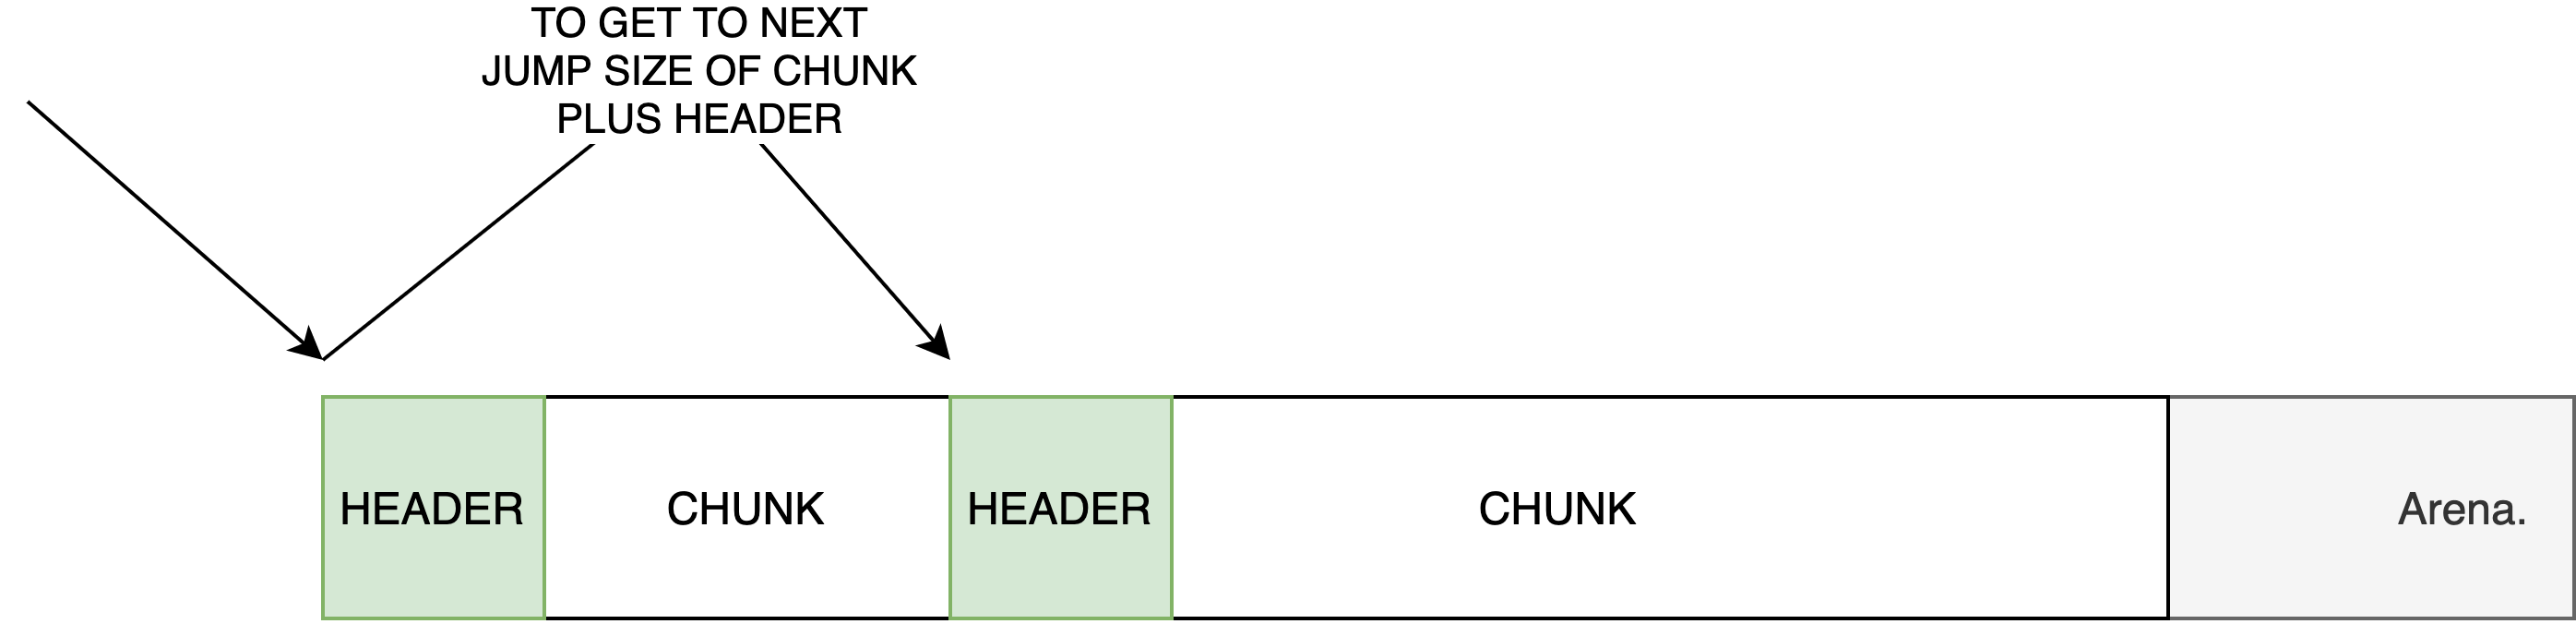
\includegraphics[scale=0.12]{images/arena-rep.png}
\end{center}

On each head we also information to make it possible to insert and remove chunks. Such as before free and if the current chunk is free. To keep track on which block are currently free we store that information in a linked list.\newline

\begin{center}
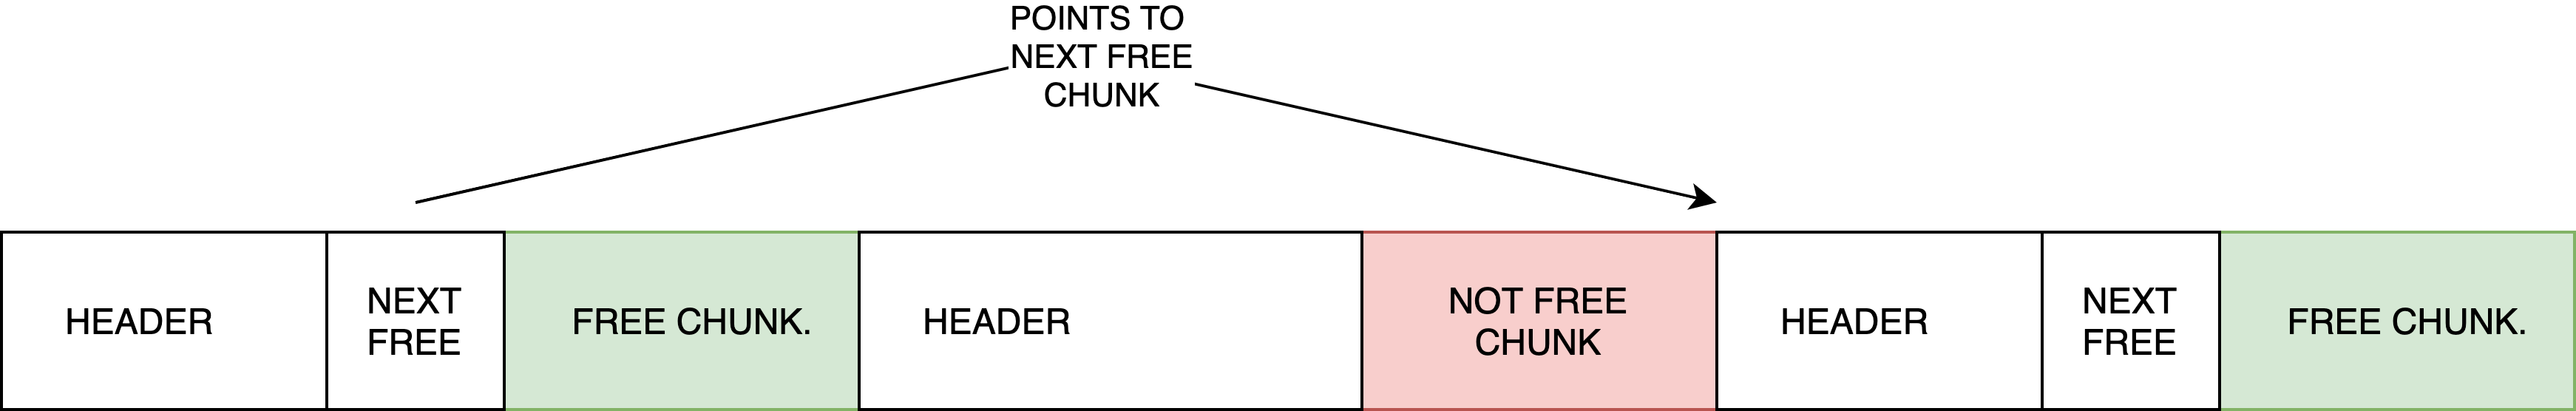
\includegraphics[scale=0.09]{images/linked-list.png}
\end{center}


Base on this we are able to both loop threw all the once which are free and we are able to free up allocated using its current size. The issue with this implementation is that this fractures up the memory in the free list. If we take for example the following code.

\lstinputlisting[
        commentstyle=\color{gray}\ttfamily,
        caption=Example of code which would fracture the arena,
        language=c,
        mathescape=true,
        morekeywords={if,then,else,return}
]{docs/example-fraction.c}



This code would create 16 bytes chunks which would fill up the arena. Even after we have free all of our chunks the sizes would remain the same and a request for a 32 bytes chunk would now not able to be full filled even though the arena is completely free.



To resolve this we implemented a merging mechanism. Which in the free list merges two chunks into one if the are after each other. This is actually really easy to done with only a couple of lines of code. All we have to do is check when freeing a block if the one before or after is free. Detach the merged block and then point from our current to the one which we have merged with. \newline

\begin{center}
    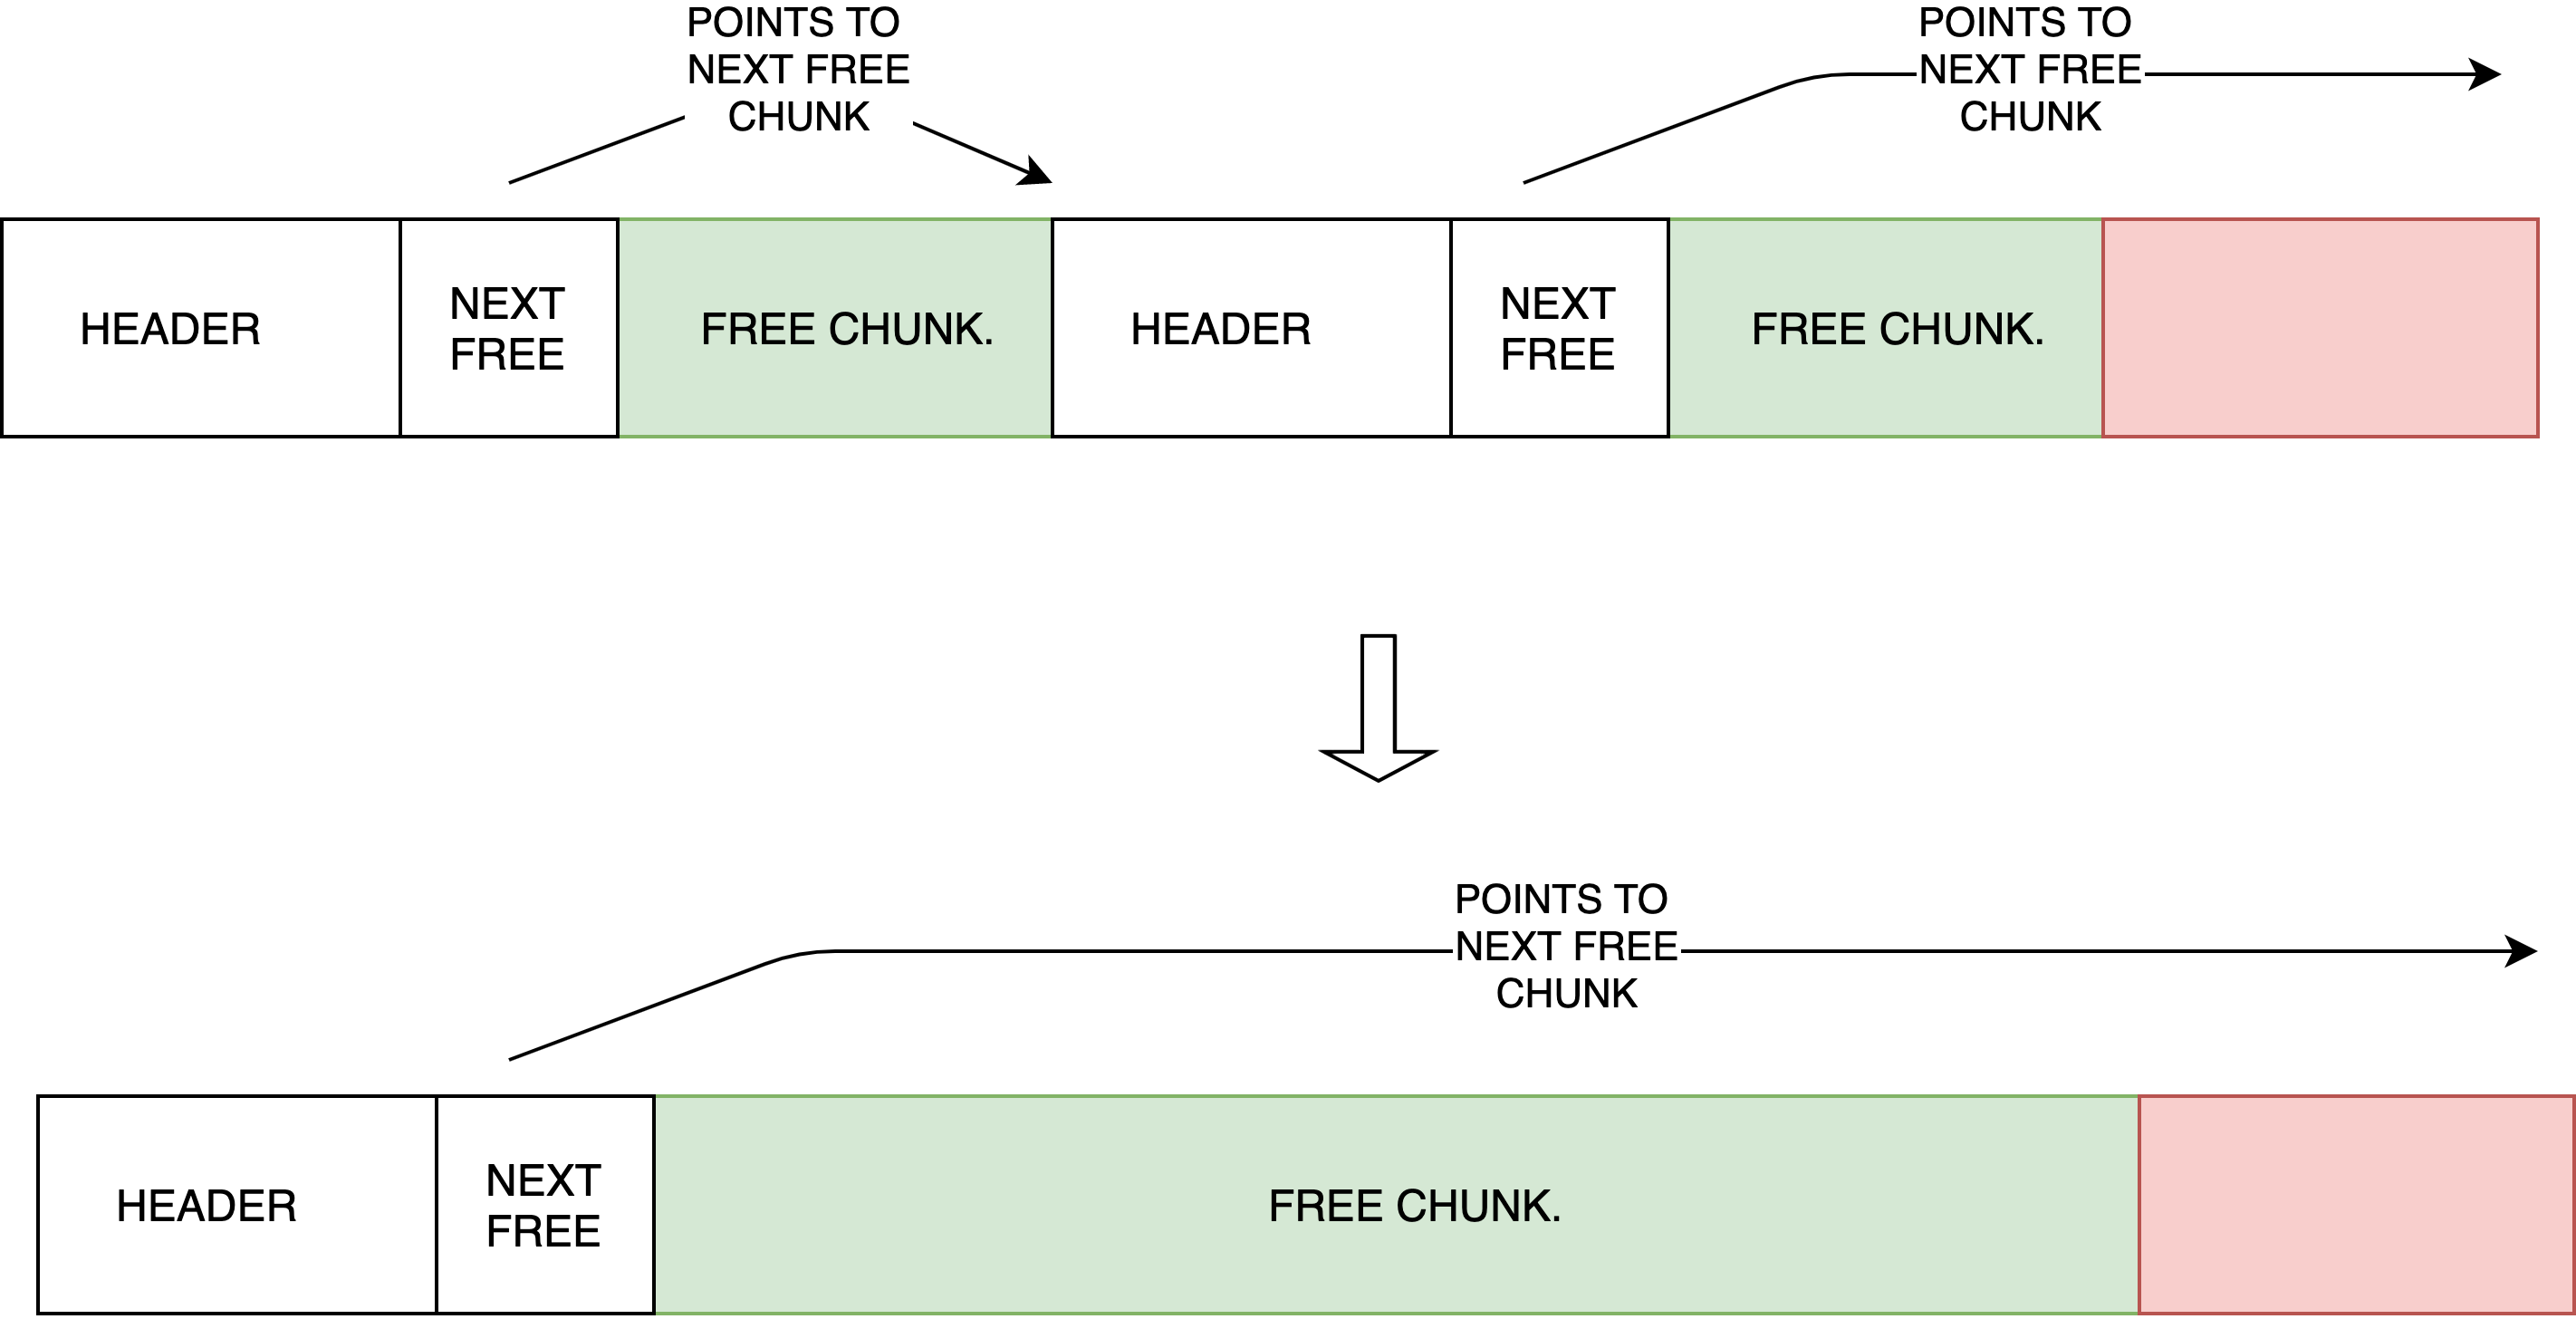
\includegraphics[scale=0.12]{images/merging-example.png}
\end{center}
     

Now looking at the code sited in \emph{Listing 1}, we are not able to allocated and free and get back to where we started, which allows us to allocated as much as we have in our free list.

Another aspect is that the time it takes to allocate a block is dependent on how long the free list is. Here we are able to see how long the list becomes when first allocates the entire list and then frees 75\% of the list.

\begin{center}
    \includegraphics[scale=0.8]{assets/free-list-size.png}
\end{center}

If it is a long free list it is going to take longer time. Therefore will merging block create a smaller list which in turns makes the program faster.


\section{Some issues we ran into}

What we had the most issues with was the initialization of the arena. We wrongly configured the sentinel which gave us undefined behaviors. Our sentinel at first was not configured to be not free which made the merging logic not work as expected. After that we did not insert the arena into the free section which gave us issues when trying to make any allocations at all. Besides those two mishaps we actually were in pretty good shape. After the initialization we were able to get threw the rest of the program without any real issues.



\section{Tests}

To test to see if our merging had an effect we wrote a small program which allocated chunks between 8 to 4096 bytes and freed them. To simulate the randomness of software we also at random freed them directly after we had 75\% of the requests be realized directly after and 25\% where released after the entire program.

\begin{center}
    \includegraphics[scale=0.8]{assets/merge-vs-no-merge.png}
\end{center}

We could explain this graph by thinking about what is going on when we merge two. Since we merge whether we are able to the length of the list will be at least cut in half!

One might wonder what would happen if we only free after we have allocated the entire list and then freed them in order. Then we would not ever be able to preform any merges and the result should look about the same for both when merging and without merging.

\begin{center}
    \includegraphics[scale=0.8]{assets/merge-vs-no-merge-same.png}
\end{center}

As we can see then the merges have little to no effect!

\section{Improvements}

For improvements we choose to remove the linked list pointers to the not free data chunks. We did this by making two real changes.

\begin{enumerate}
    \item When allocating a memory chunk return an address which is offset back the size of two head pointers. This will make it so that program will override the pointers with usable data.
    \item When using \emph{after} and \emph{before} we need to take into account if it is a free block or a allocated block. 
\end{enumerate}



\begin{center}
    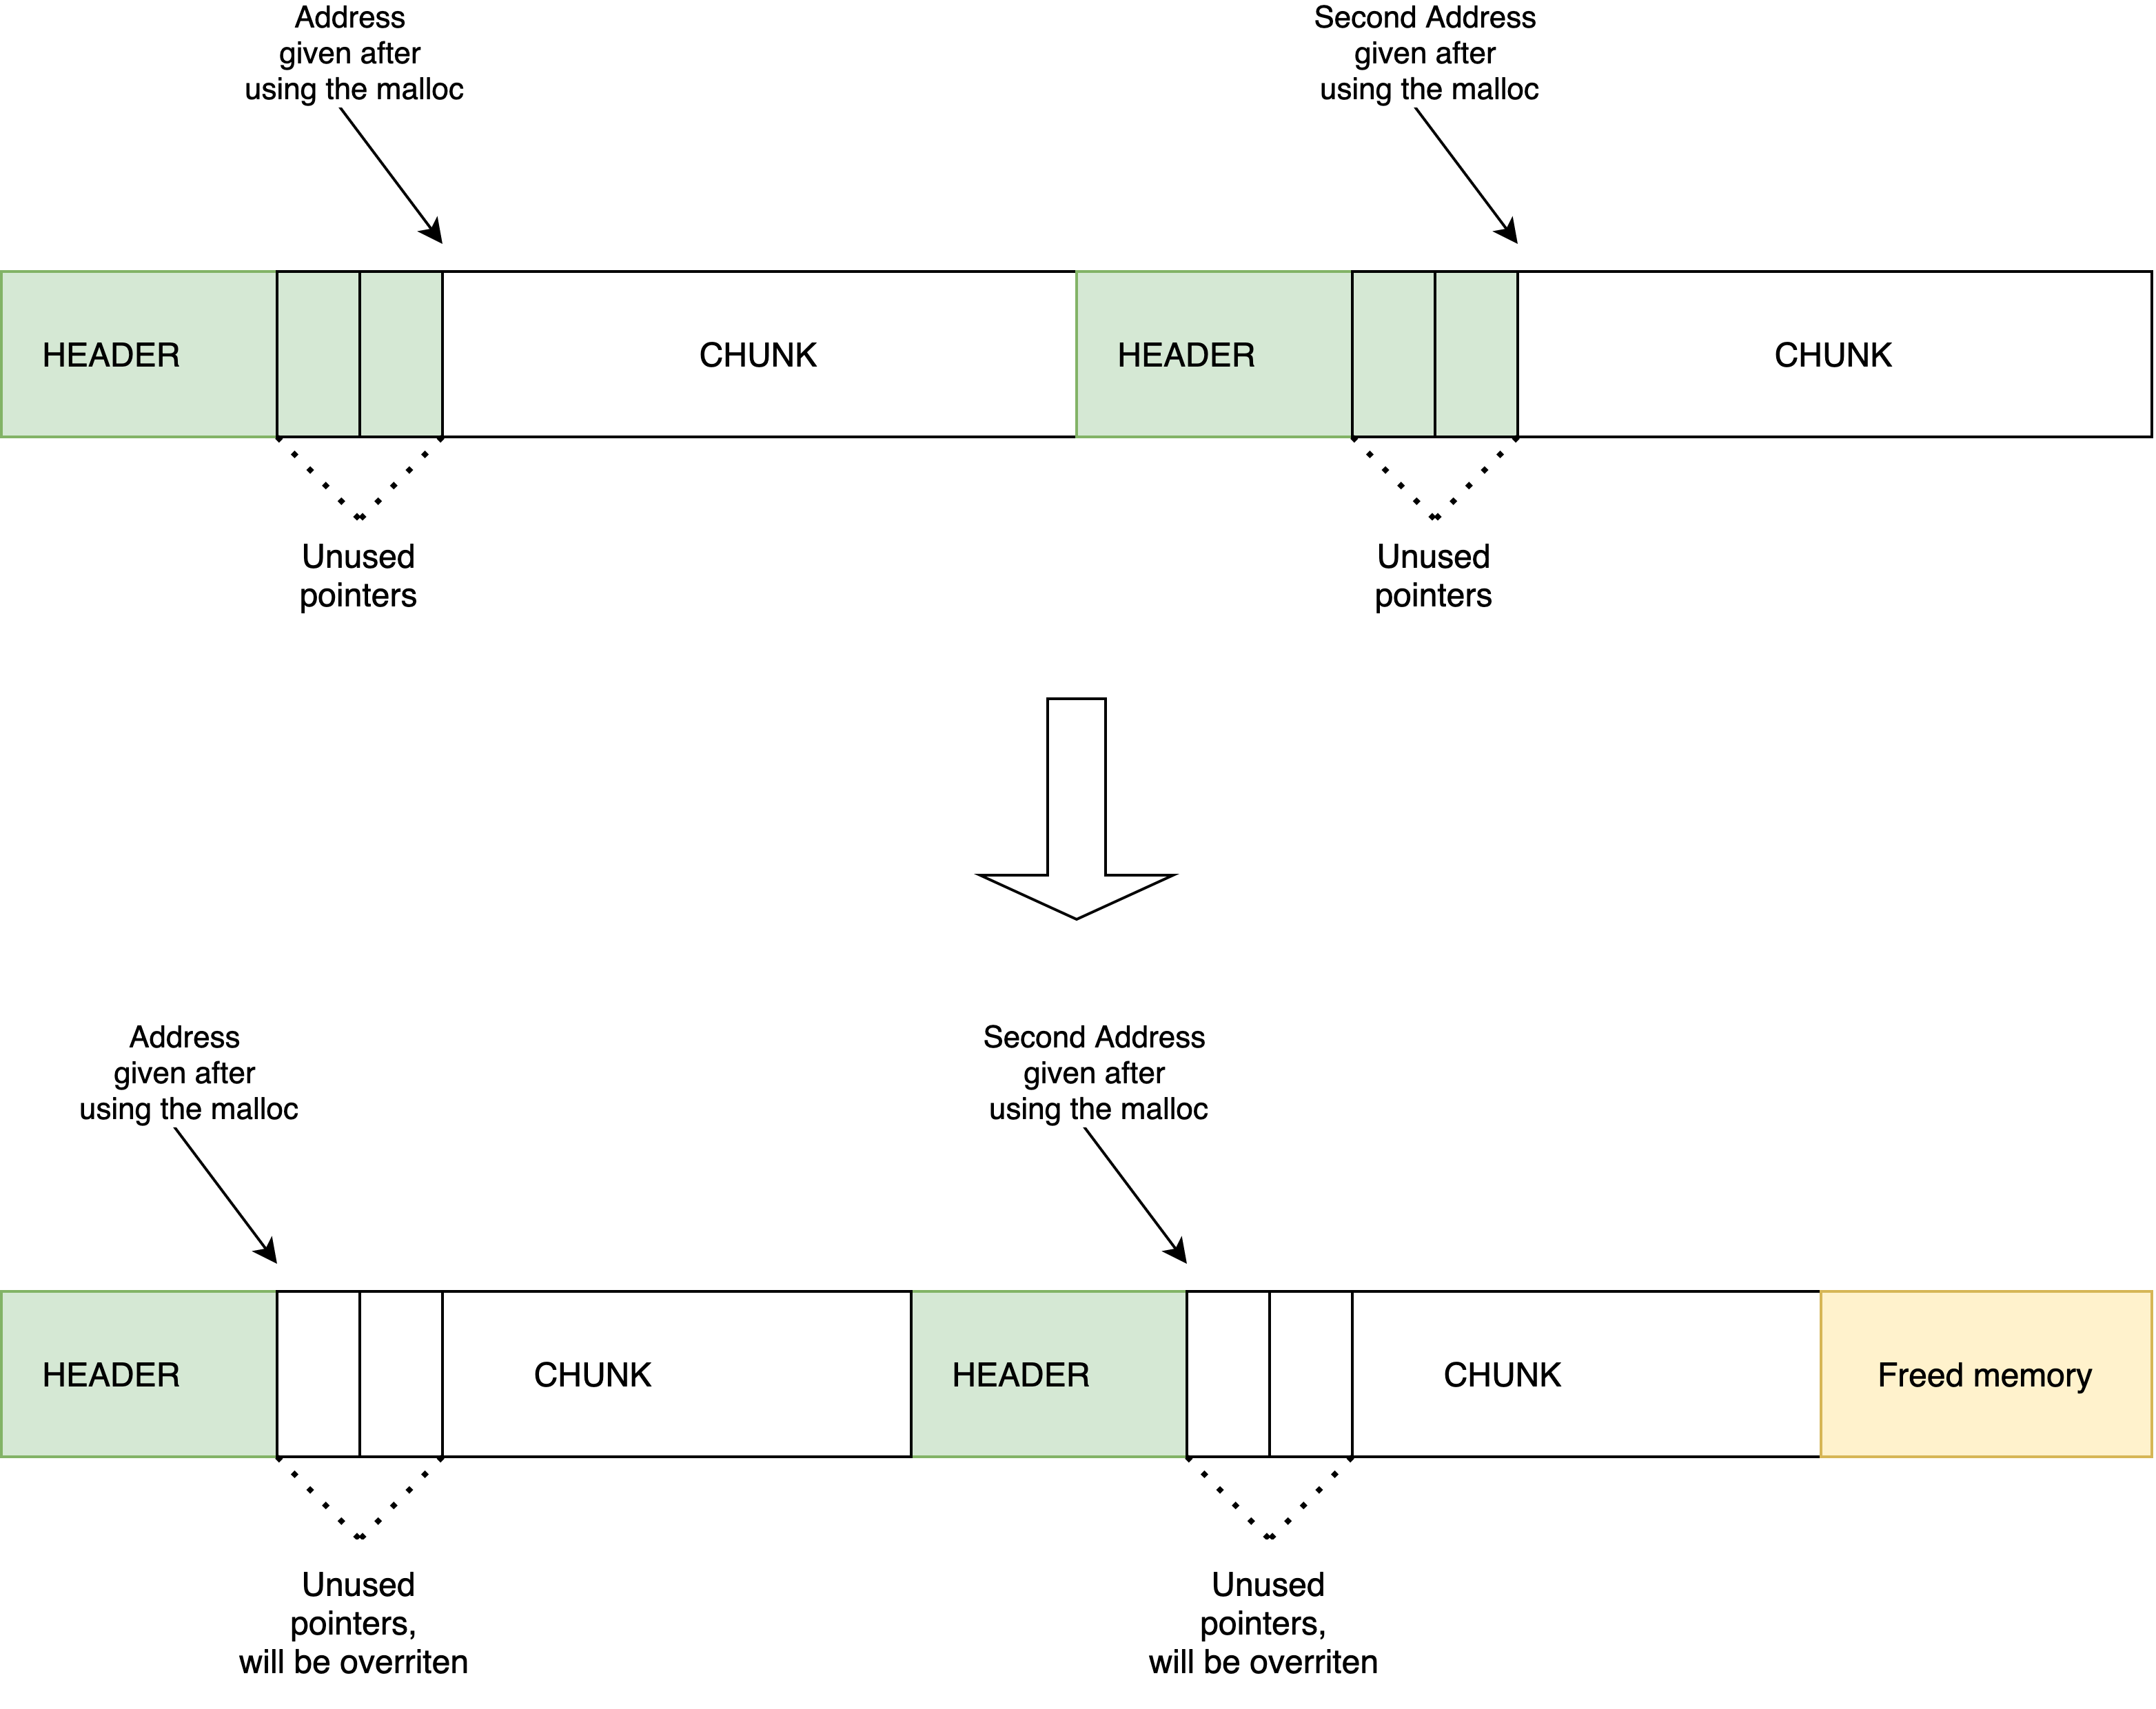
\includegraphics[scale=0.12]{images/no-pointer-on-taken.png}
\end{center}
     
     
This cut the size of the header of a taken block from 32 bytes to 16 bytes. Since we use merge logic only on the free blocks we are more likely to have more taken blocks than freed block making this improvement very important. 
However this does not any notable effect on time complexity since this does not affect the length of the freed list and the look up from the previous is still in \emph{O(1)}.

\begin{center}
    \includegraphics[scale=0.8]{assets/ptr-vs-no-ptr.png}
\end{center}

\section{Source code}


\emph{https://github.com/erikschmutz/ID1206/tree/main/lab2-malloc}

\end{document}


